\subsection{Datenflüsse}
\label{app:Datenfluesse}
\begin{figure}[htb]
    \centering
    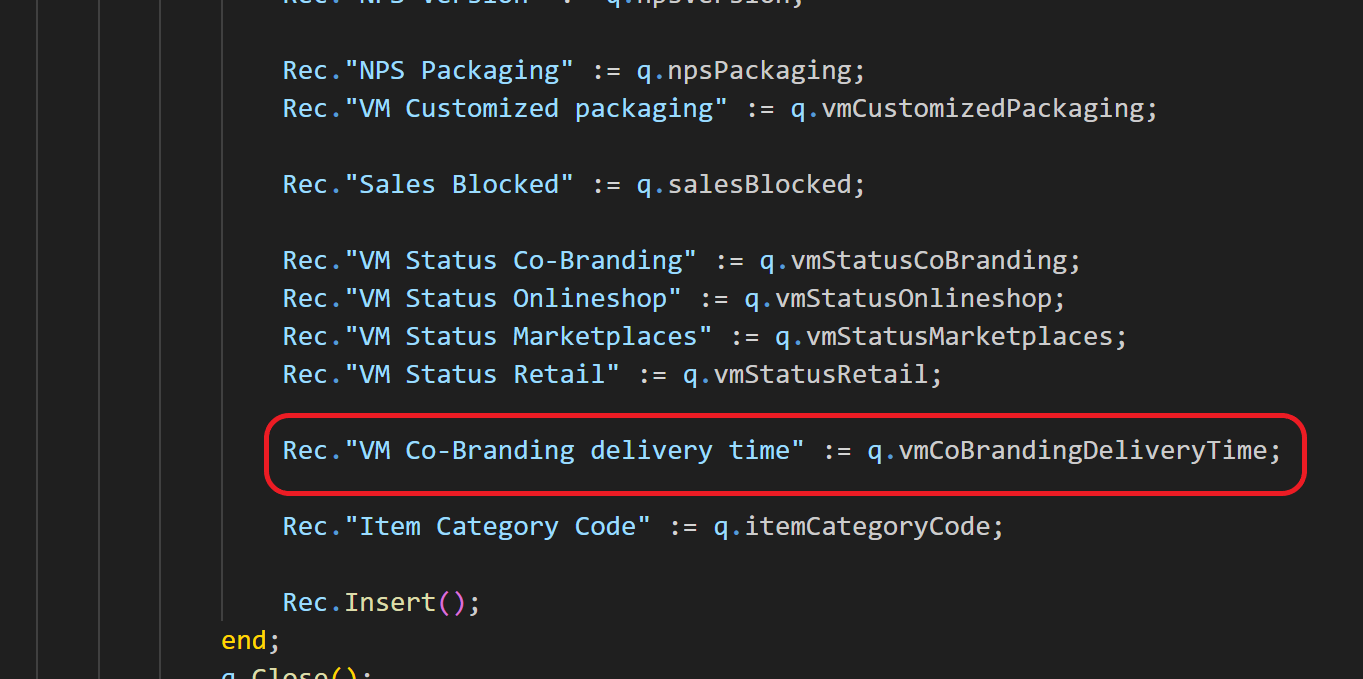
\includegraphics[width=0.6\textwidth]{page 57129 VM CRM Quote Item.png}
    \caption{virtuelle Tabelle, um die Daten aus CRM abzurufen und in BC anzuzeigen.}
    \label{fig:page 57129 VM CRM Quote Item}
\end{figure}
\begin{figure}[htb]
    \centering
    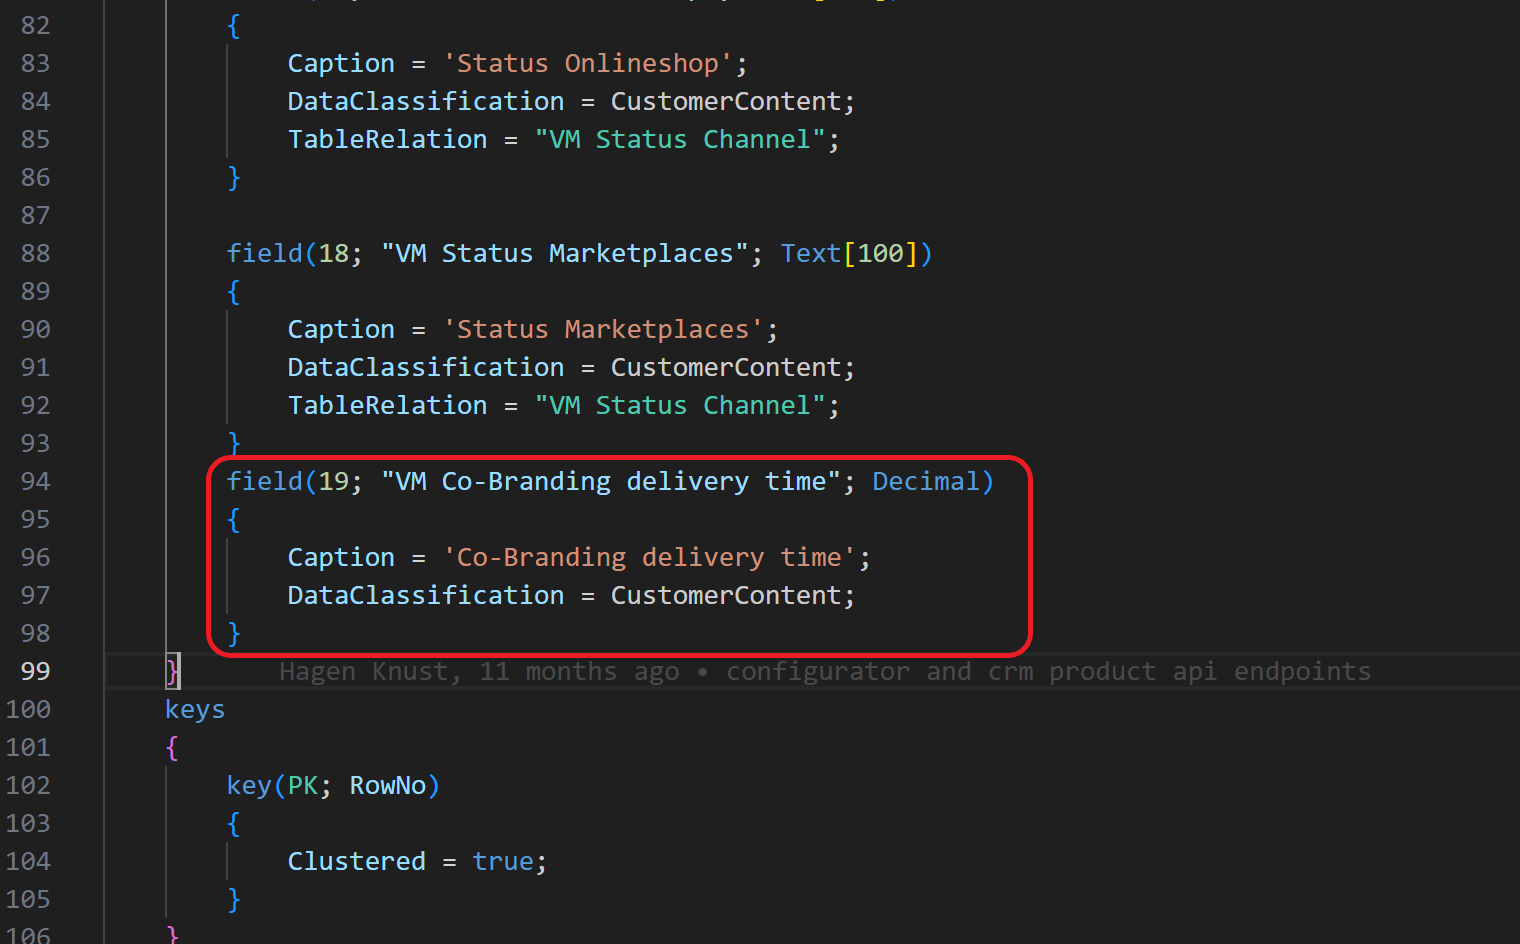
\includegraphics[width=0.6\textwidth]{table 57111 VM CRM Quote Item.png}
    \caption{temporäre Tabelle mit Feldern zur Angebotserfassung im CRM}
    \label{fig:table 57111 VM CRM Quote Item}
\end{figure}
\begin{figure}[htb]
    \centering
    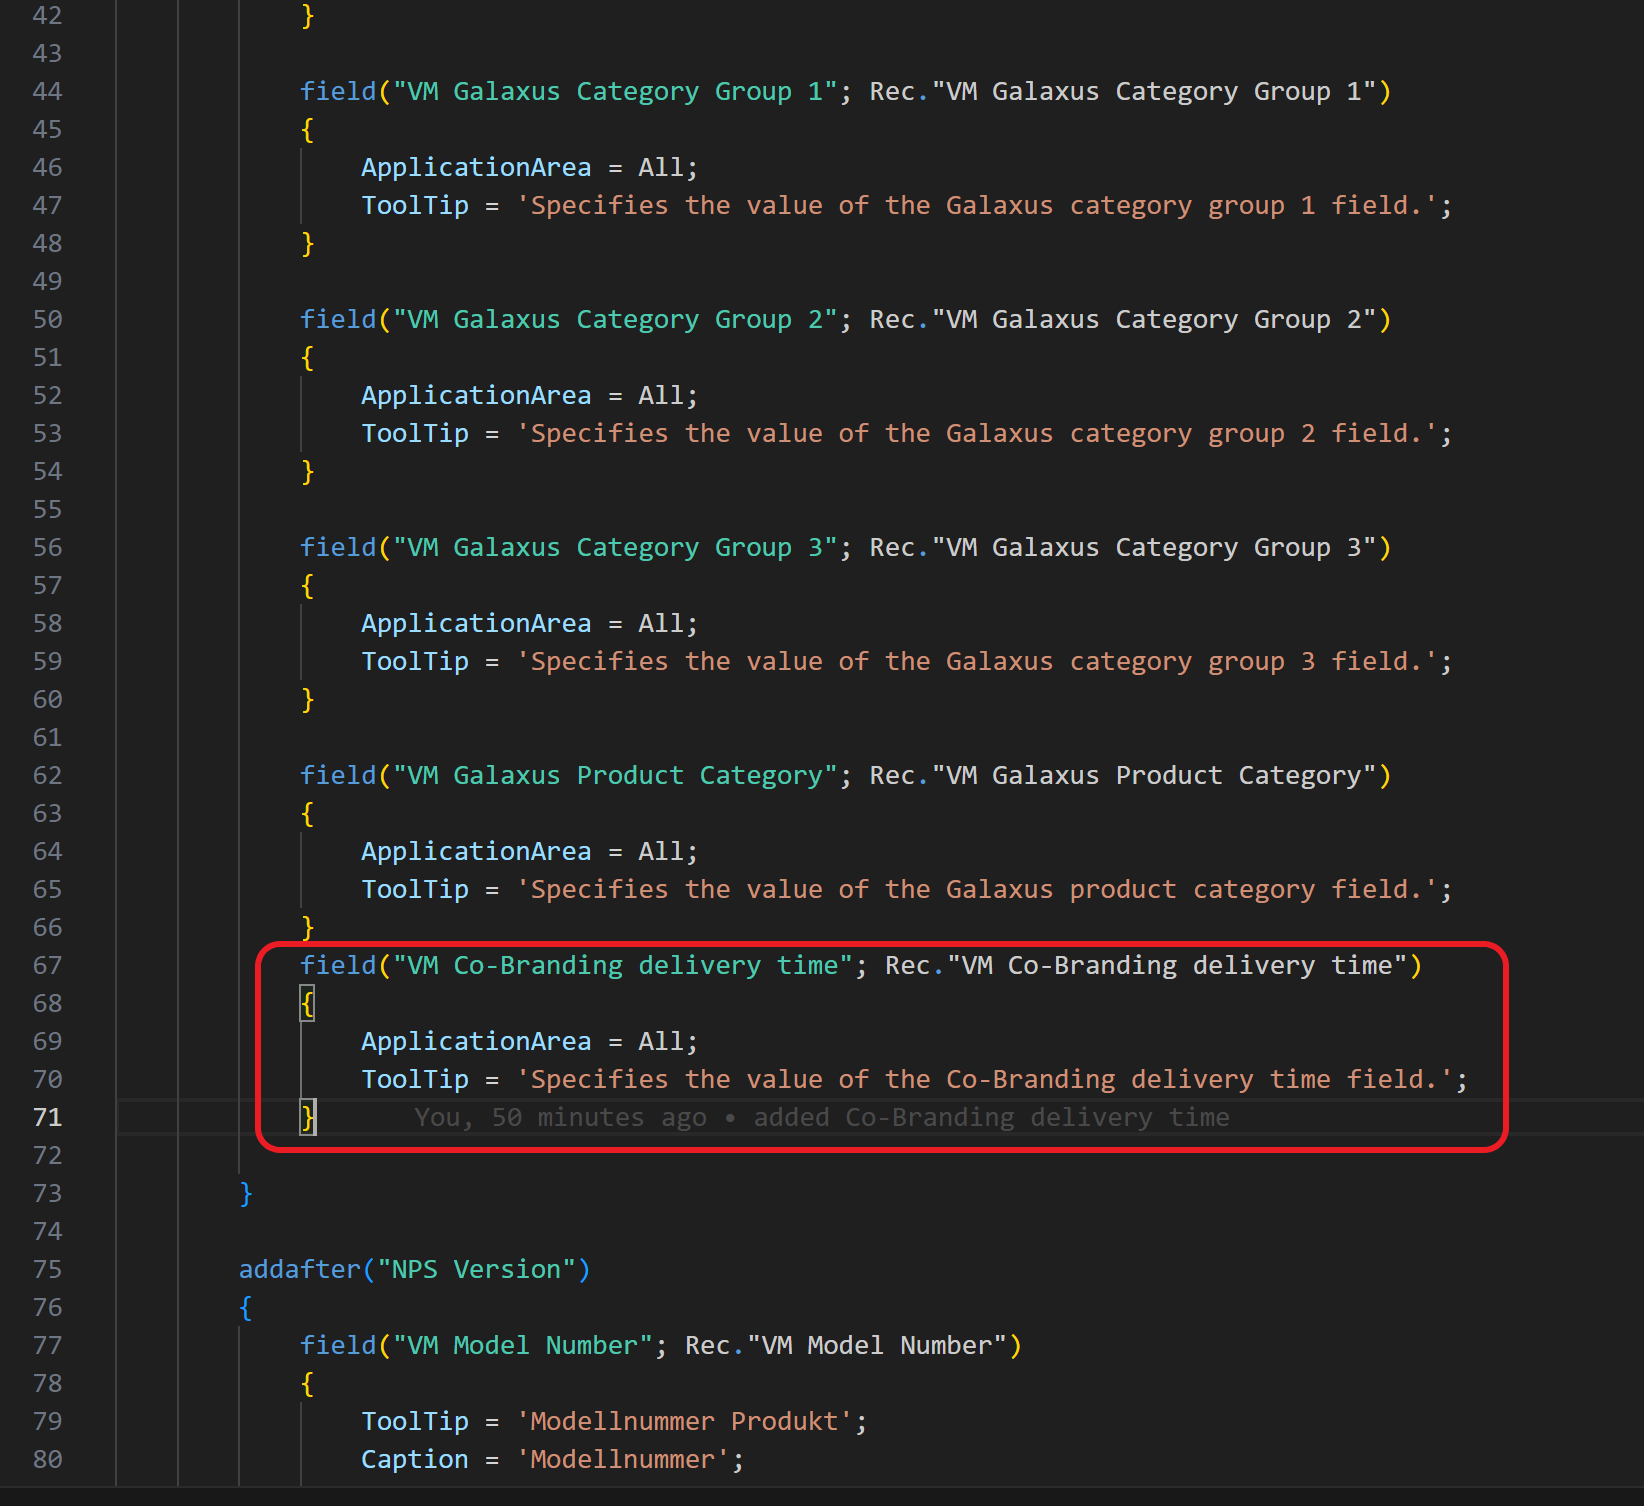
\includegraphics[width=0.6\textwidth]{pageextension 57108 VM Item Card extends.png}
    \caption{Felddefinitionen für die Erweiterung der Artikelkarte in BC.}
    \label{fig:pageextension 57108 VM Item Card extends}
\end{figure}
\begin{figure}[htb]
    \centering
    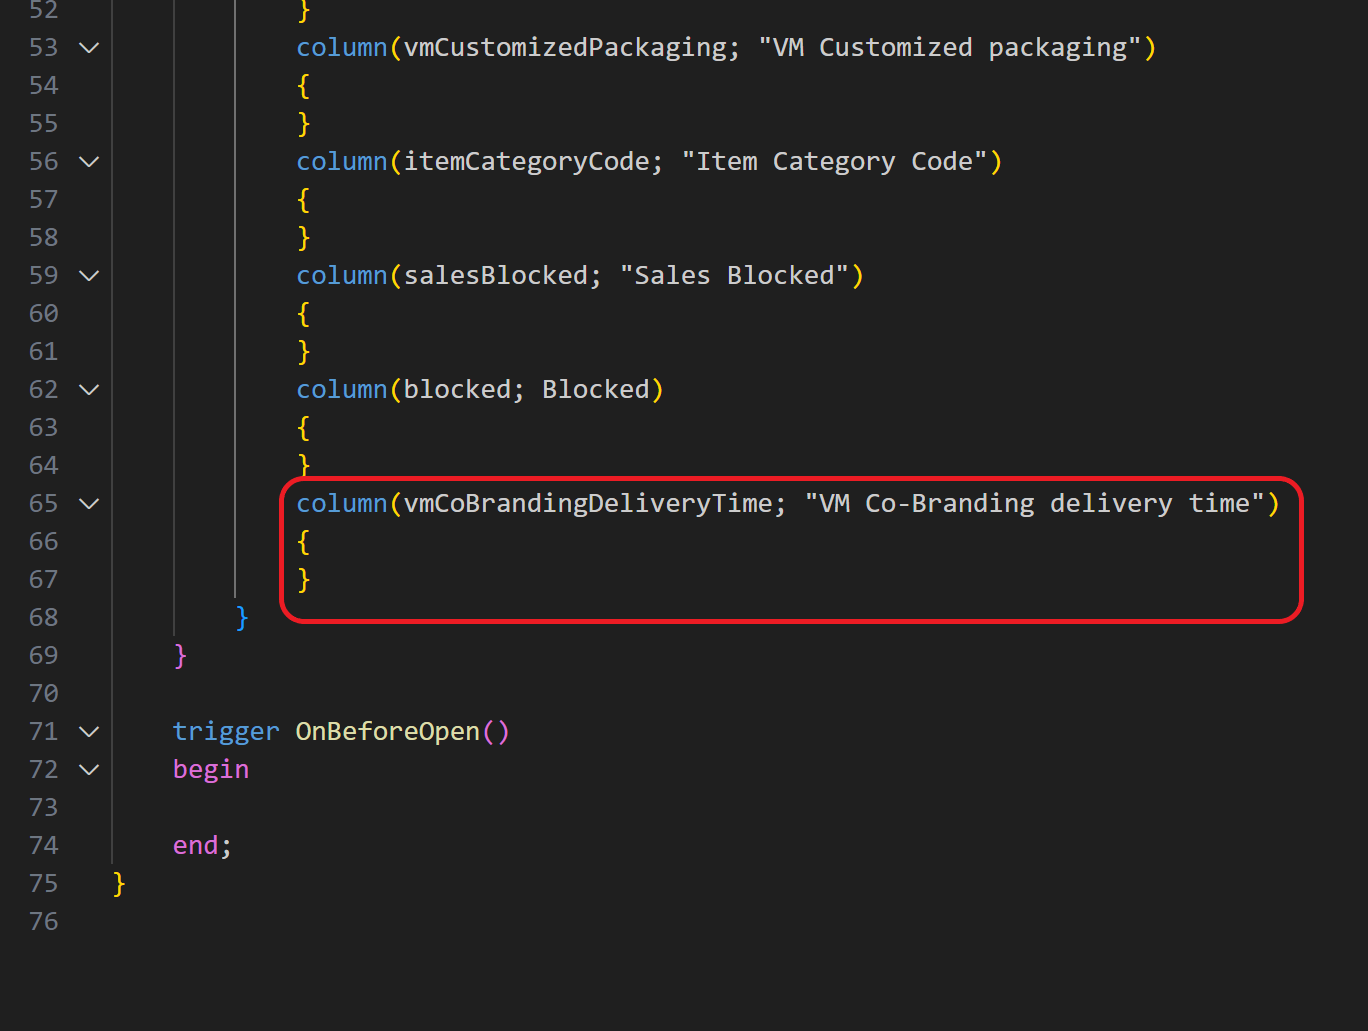
\includegraphics[width=0.6\textwidth]{query 57110 VM CRM Quote Item.png}
    \caption{AL-Abfrage, die spezifische Daten zu einem Zitatselement
    in CRM abruft und Filter anwendet, um die zurückgegebenen Ergebnisse zu steuern.}
    \label{fig:query 57110 VM CRM Quote Item}
\end{figure}
\begin{figure}[htb]
    \centering
    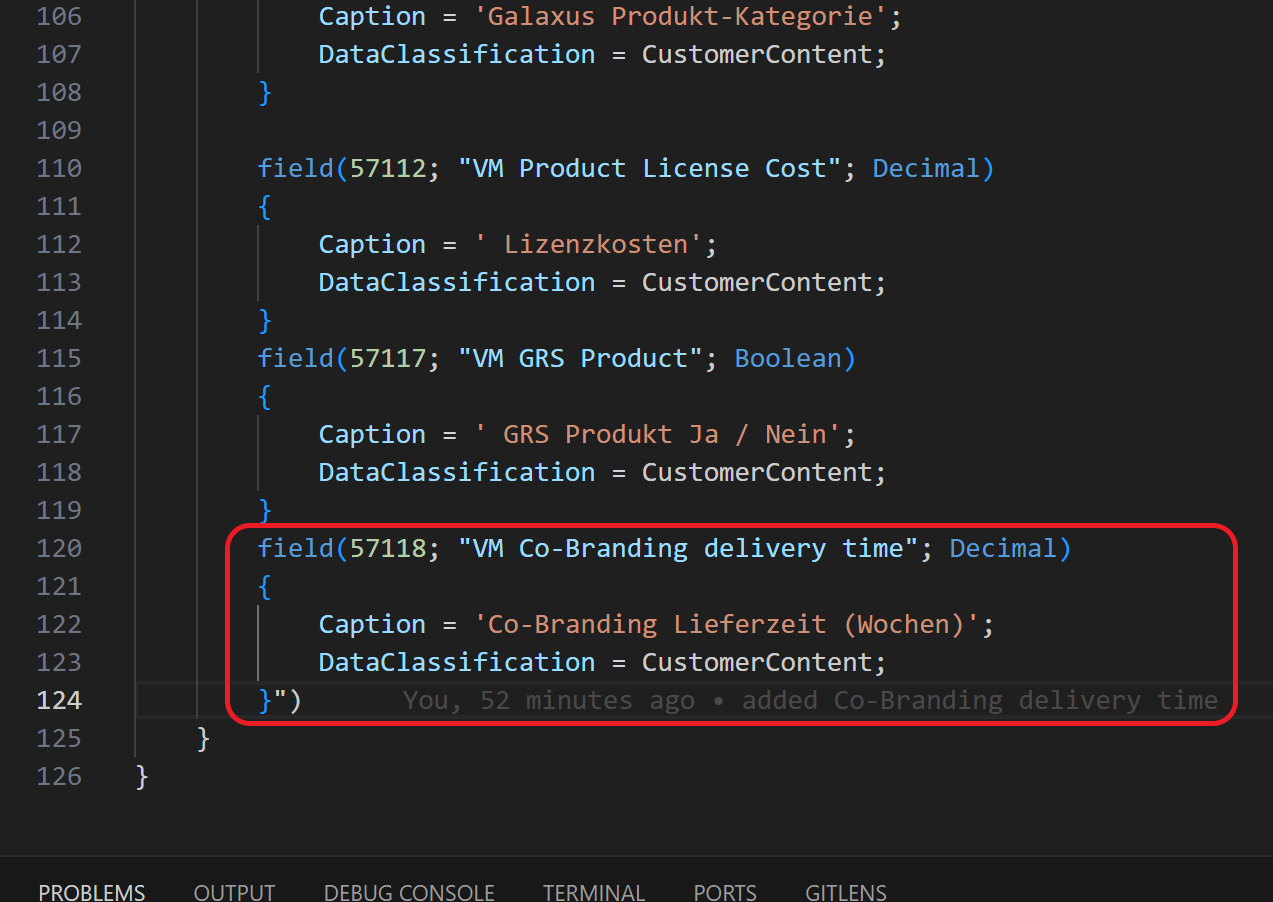
\includegraphics[width=0.6\textwidth]{tableextension 57109 VM Item.png}
    \caption{Tabellenerweiterung um Felder zur Item-Tabelle hinzuzufügen, die Informationen zur VM Items enthalten.}
    \label{fig:tableextension 57109 VM Item}
\end{figure}
\begin{figure}[htb]
    \centering
    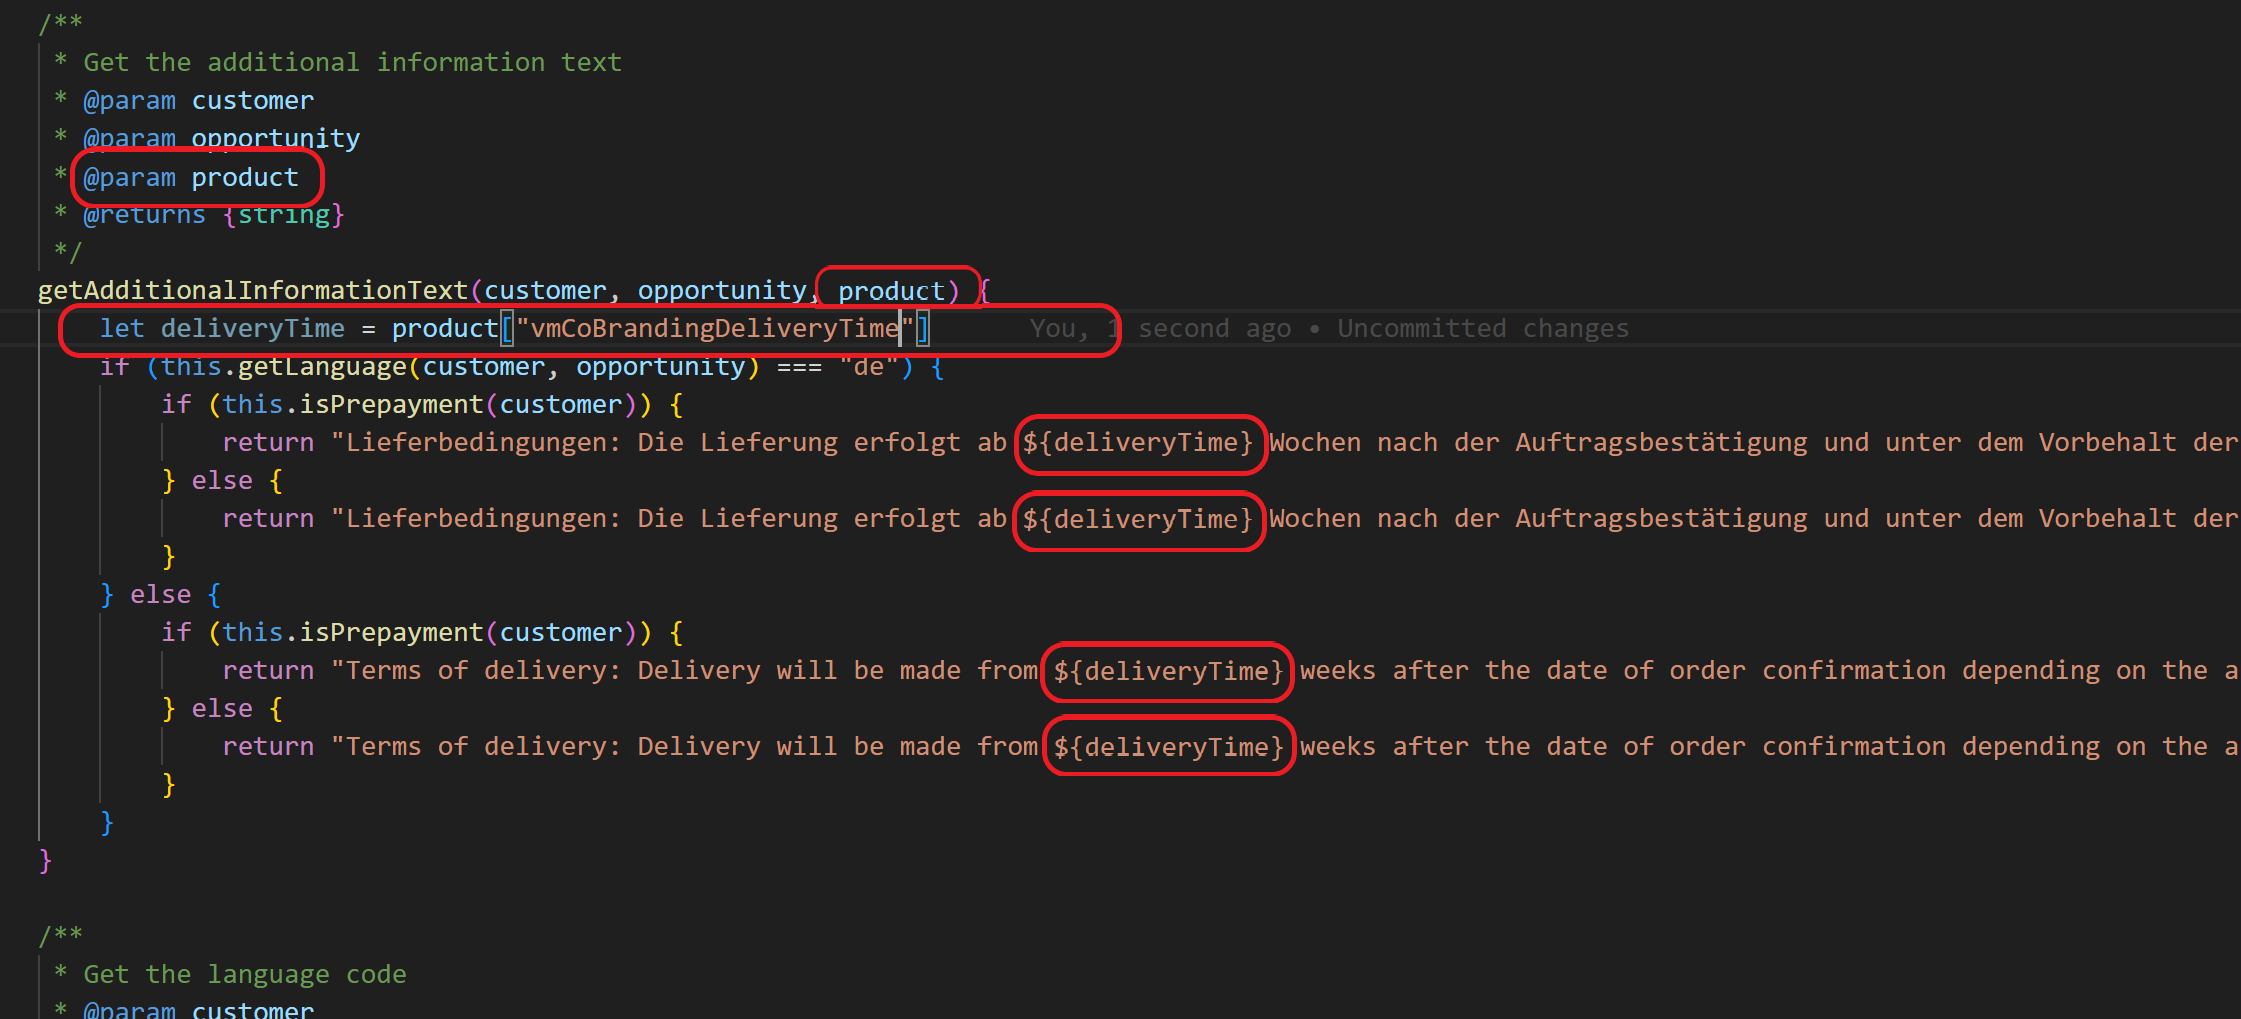
\includegraphics[width=0.6\textwidth]{opportunity.js.png}
    \caption{Lieferbedingungstext basierend auf Kunden-, Opportunitäts- und Produktinformationen.}
    \label{fig:opportunity.js}
\end{figure}
\clearpage